\cotefile{48}
\scanpage{2}
\noindent\hfill Plan EGA $\overline{\text{\uline{VI}I}}$

% archive sheet number: 1
\clearpage
\scanpage{3}
\noindent EGA \uline{Chap.\ $\overline{\mathrm{\unsure{VI|VII}}}$}\qquad
\uline{\unsure{Schémas} en \unsure{gpes|groupes} et \deleted{\unsure{fibrés} \unsure{principaux} \unsure{homogènes}} \inserted{Torseurs}}

\noindent\textcircled{A}\quad \uline{Propriétés générales}

\noindent\uline{\S~1}\quad \unsure{Histoires|Histoire} \unsure{de|des|du} passage d'un \unsure{pt} à \unsure{tout|tous}, de propriétés ouvertes / propriétés générales des morphismes

\noindent\uline{\S~2}\quad \unsure{Composante|Composantes} neutre. \unsure{Dimensions|Dimension}. Séparation

\noindent\uline{\S~3}\quad Groupes affines

% slanted
\reversemarginpar
\noindent\margin{\raggedleft\shortstack[r]{sur\\un \unsure{corps}}\,$\Biggl\{$}\uline{\S~4}\quad Sous-gpes engendrés
\normalmarginpar

\noindent\uline{\S~5}\quad Passage au quotient: \inserted{\deleted{(sur un corps)}}\unsure{espaces} hom. et gpes quotients.

\noindent\uline{\S~6}\quad $G^{\unsure{\tau|t}}$ \unsure{si} $\unsure{G|C}$ \unsure{comm} (cf \unsure{TDTE} $\overline{\text{\uline{VI}}}$ n\textsuperscript{\uline{o}}~1)

\noindent\textcircled{\deleted{B}B}).\quad \uline{Études infinitésimales}

\noindent\S~7\quad \unsure{Questions|Question} d'extensions infinitésimales. (cf SGAD $\overline{\text{\uline{II}}}$)

\noindent\S~8\,: \quad \unsure{Hyperalgèbre|Hyperalgèbres} d'un groupe alg. et \unsure{op.|gr.} diff \unsure{inv|inv.}

\noindent\S~9.\quad \unsure{Frobeniusiennes|Frobeniusienne|Frobeniusien}

\noindent``\S~10''\quad \deleted{\unsure{Alg|Algè}} Groupes \unsure{radiciels} et $p$-algèbres de Lie

\noindent\inserted{\S~11\quad Dualité de Cartier.}

\noindent\deleted{\textcircled{\unsure{C}}\quad \S.\quad \uline{Dualité de Cartier}}

\noindent\textcircled{C}\quad \uline{Groupes de \unsure{t.} \unsure{m.}}\ ; \uline{propriétés de rigidité liées aux \unsure{pts} d'ordre \unsure{fini}.}

\noindent\S~12.\quad \unsure{Maximum} : SGAD $\overline{\text{\uline{VIII}}}$, $\overline{\text{\uline{IX}}}$, $\overline{\text{\uline{X}}}$

% archive sheet number: 2
\clearpage
\scanpage{4}
\mspage{(30}
\begingroup
\reversemarginpar
\makeatletter\tagsleft@true\makeatother
\noindent\margin{\handwritten{$\varphi\qquad \unsure{\varepsilon|\mathcal{E}|\mathscr{E}}_{\xi'}$}}%
\handwritten{\tikz[baseline=-.2ex]{\draw (0,0) .. controls (.13,.16) and (.36,.24) .. (.43,.21) .. controls (.45,.19) and (.45,.17) .. (.45,.16);}}\,
Lorsque $\handwritten{\varphi}$ est de la forme $\handwritten{\varepsilon_{\deleted{\unsure{\xi'|\xi}}\xi'}}$, donc
\margin{\handwritten{$\varphi$}}
\[
\handwritten{\varphi} \handwritten{\simeq} \mathop{\underset{\handwritten{\longrightarrow}}{\mathrm{lim}}}\limits_j {X'_j}^{\handwritten{\unsure{\vee|v}}}\ , 
\]
on a donc une bijection naturelle
\margin{\handwritten{$\varepsilon_{\xi}\quad\varepsilon_{\xi'}\qquad .$}}
\[
\operatorname{Hom}\bigl(\handwritten{\varepsilon_{\deleted{\unsure{\xi}}\xi}},\handwritten{\varepsilon_{\deleted{\unsure{\xi}}\xi\unsure{'}}} ,\bigr)
 \handwritten{\simeq} \mathop{\underset{\handwritten{\longleftarrow}}{\mathrm{lim}}}\limits_i \mathop{\underset{\handwritten{\longrightarrow}}{\mathrm{lim}}}\limits_j \operatorname{Hom}_{X}(X'_j,X_i)\handwritten{\deleted{\unsure{,|.}}}\qquad .
\tag*{$(*)$}
\]

\noindent D'autre part on a (dans la catégorie des préschémas)
\margin{\handwritten{$\deleted{\unsure{\xi}}$}}
\[
\bar X(\handwritten{\xi}) == \mathop{\underset{\handwritten{\longleftarrow}}{\mathrm{lim}}}\limits_i X_i\handwritten{\deleted{\unsure{\xi}}}\ ,\quad
\bar X(\handwritten{\xi}') = \mathop{\underset{\handwritten{\longleftarrow}}{\mathrm{lim}}}\limits_j X'_j\ ,
\]
d'où
\[
\handwritten{\unsure{-}}\; \operatorname{Hom}_{X}(\bar X(\handwritten{\xi}'),\bar X(\handwritten{\xi})) \handwritten{\simeq}
 \mathop{\underset{\handwritten{\longleftarrow}}{\mathrm{lim}}}\limits_i \operatorname{Hom}_{X}(\bar X(\handwritten{\xi}'),X_i)\ ,
\]
\margin{\handwritten{\tikz{\draw (0,0) .. controls (.04,.18) and (.27,.10) .. (.49,.28) .. controls (.58,.35) and (.56,.45) .. (.54,.47);}}}
d'autre part, comme $X_i$ est loc\inserted{\handwritten{\tikz[baseline=(w.base)]{%
\node[anchor=base west,rotate=14,inner sep=.3pt] (w) at (0,0) {alement};
\draw (-.04,-.17) .. controls (-.01,.08) and (.42,.04) .. (.85,.27) .. controls (.98,.34) and (1.04,.41) .. (.99,.42);
}}} de présentation finie sur $X$\handwritten{, on a}
\[
\operatorname{Hom}_{\handwritten{X}}(\bar X(\handwritten{\xi}'),X_i) \handwritten{\simeq}
 \mathop{\underset{\handwritten{\longrightarrow}}{\mathrm{lim}}}\limits_j \operatorname{Hom}_{X}(X_j,X_i)\handwritten{,}
\]
d'où
\[
\operatorname{Hom}_{X}(\bar X(\handwritten{\xi}'),\bar X(\handwritten{\xi})) \handwritten{\simeq}
 \mathop{\underset{\handwritten{\longleftarrow}}{\mathrm{lim}}}\limits_i \mathop{\underset{\handwritten{\longrightarrow}}{\mathrm{lim}}}\limits_j \operatorname{Hom}_{X}(X'_j,X_i)\ .
\tag*{$(**)$}
\]

\noindent La comparaison de $(*)$ est $(**)$ donne la\handwritten{$\mid$}conclusion voulue (moyennant une verification de compatibilités, laissé\deleted{\unsure{n|e|s}}e au lecteur).

% slanted
\noindent\margin{\handwritten{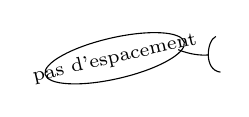
\begin{tikzpicture}[baseline,scale=.84]
\node[rotate=13,inner sep=1pt] (m) at (0,0) {\scriptsize\unsure{pas} d'\unsure{espacement}};
\draw[rotate=13] (0,0) ellipse [x radius=1.08cm,y radius=.31cm];
\draw (.96,.13) .. controls (1.13,.06) and (1.29,.04) .. (1.42,.05);
\draw (1.53,.33) .. controls (1.39,.27) and (1.34,-.18) .. (1.60,-.21);
\end{tikzpicture}}}%
b) \uline{Le foncteur envisagé est essentiellement surjectif:}

\noindent 7.9.1.\quad Remarquons d'abord que si $C$ est un site où les $\mathop{\underset{\handwritten{\longleftarrow}}{\mathrm{lim}}}\limits$ finies sont représentable, $\handwritten{\widetilde}{C} = \underline{E}$ le topos correspondant alors\handwritten{,} tou\deleted{s}\handwritten{t}%
\margin{\handwritten{,\quad t}}
foncteur\deleted{s} fibre\deleted{s} $\handwritten{\deleted{\unsure{\xi|\varphi}}\varphi}$ sur $\underline E$ peut se représenter comme une ``limite''
\margin{\handwritten{$/\quad /\quad\varphi$}}
inductive pseudo-filtrante connex\deleted{\unsure{e}}\handwritten{e}\handwritten{''} d\deleted{\unsure{e}}\handwritten{e} foncteurs de la forme
\margin{\handwritten{e\quad e}}
\margin{\handwritten{$]\,[ $}}
\[
\handwritten{\check}{Y}(F) == F(Y) = \operatorname{Hom}(\handwritten{\widetilde}{Y},F),\handwritten{\big]\big[}\, Y\handwritten{\in}\operatorname{Ob} C\handwritten{,}
\]
(ou $\handwritten{\widetilde}{Y}$ est le faisceau associé à $Y$)\handwritten{,} de la façon suivante. On considèr\deleted{\unsure{e|s}}\handwritten{e}
\margin{\handwritten{,}}
la catégorie\handwritten{$\mid C_{\deleted{\unsure{\xi|\varphi}}\varphi}$} des couples $(Y,\handwritten{\xi})$, avec $Y\handwritten{\in}\operatorname{Ob} C$, $\handwritten{\xi}\handwritten{\in\varphi}(\handwritten{\widetilde}{Y})$
\margin{\handwritten{$C_{\varphi}$}}
\endgroup

% archive sheet number: 3
\clearpage
\scanpage{5}
\noindent\tikz[baseline=(n.base)]{\node[inner sep=0pt] (n) {D};\draw (n.center) ellipse (.82em and .88em);\draw (n.center) ellipse (1.08em and 1.13em);}\quad
\uline{Propriétés générales des} \uline{\unsure{schémas} \unsure{abéliens|abeliens}} \uline{et \unsure{parabeliens|parabéliens|paraabeliens|paraabéliens}}

\figure{\makebox[\linewidth][l]{\hspace*{3em}\tikz{\foreach \y in {0,.12,.24,.36,.48}{\fill (0,\y) ellipse (.012 and .020);}}}}

\noindent\tikz[baseline=(n.base)]{\node[inner sep=0pt] (n) {E};\draw (n.center) ellipse (.68em and .96em);\draw (n.center) ellipse (.88em and 1.12em);}\quad
\uline{Extensions des schémas \unsure{abéliens|abeliens} par \unsure{gpes|groupes} affines}

\noindent\hspace*{7em} (th. de \unsure{Chevalley}....).

\figure{\makebox[\linewidth][l]{\hspace*{3em}\tikz{\foreach \y/\l in {0/.08,.13/.04,.26/.06,.39/.06,.52/.09}{\draw (0,\y) -- ++(0,\l);}}}}

\noindent%
\figure{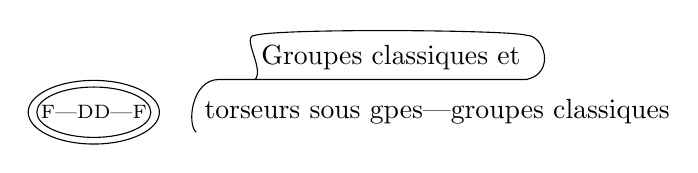
\begin{tikzpicture}[baseline=(t.base)]
\node[anchor=base,font=\scriptsize] (letter) at (-1.40,0) {\deleted{\unsure{F|D}}\unsure{D|F}};
\draw (letter.center) ellipse (2.06em and .91em);
\draw (letter.center) ellipse (2.37em and 1.15em);
\node[anchor=south west,inner xsep=2pt] (ins) at (.65,.50) {\inserted{Groupes classiques et}};
\draw (ins.south west) .. controls +(.12,.14) and +(-.19,0) .. (ins.north west)
  .. controls +(.30,.09) and +(-.20,.07) .. (ins.north east)
  .. controls +(.23,0) and +(.37,.08) .. (ins.south east) -- (ins.south west);
\draw (ins.south west) -- (.19,.50) .. controls (-.16,.50) and (-.22,-.07) .. (-.10,-.17);
\node[anchor=base west,inner sep=0pt] (t) at (0,0) {\uline{torseurs sous \unsure{gpes|groupes} classiques}};
\end{tikzpicture}}\margin{(N'importe \unsure{où|ou})}

\noindent\hfill et théorème de l'\unsure{isotrivialité} sur un corps \unsure{(?)|(!)|(P.)}.

\noindent\tikz[baseline=(n.base)]{\node[inner sep=0pt] (n) {\scriptsize\deleted{\unsure{E|F}}\unsure{F|E}};\draw (n.center) ellipse (2.20em and .95em);\draw (n.center) ellipse (2.40em and 1.18em);}\quad
Modèles de \unsure{Néron|Neron} (?)

\noindent\hfill Un \unsure{paragraphe} de \unsure{variations} sur le ``th. \unsure{du|des} carré''?

\noindent Réf\quad \begin{tabular}[t]{@{}l@{}}
SGAD\\
BIBLE\\
``Boulder''\\
Livre(s) Mumford
\end{tabular}

% archive sheet number: 4
\clearpage
\scanpage{6}
\mspage{(29}
\begingroup
\makeatletter\tagsleft@true\makeatother
\[
\underline{\mathrm{Pt}}(X)^{\unsure{\circ|o|0}}\dashrightarrow
\underline{\mathrm{Pt}}(\handwritten{\widetilde}{X_{\text{ét}}})\ ,
\tag*{$(*)$}
\]
où le premier membre est défini dans 7.6.. Ceci posé, on a le

\noindent\uline{Théorème} 7.9.\quad Soit $X$ un préschéma. Le foncteur précédent $(*)$ est une \uline{an\deleted{\unsure{it|ti}}\handwritten{ti}-équivalence} de la catégorie des points géomètriques sur $X$ (avec comme morphismes les flèches des spécialisation) avec la catégorie des foncteurs fibres sur le topos étale $\handwritten{\widetilde}{X_{\text{ét}}}$.

Comme ce théorème ne servira plus dans la suite du séminaire nous nous bornons ici à une esquisse de démonstration, où nous nous permettrons certaines libertés avec les questions d'Univers.

a) \uline{Le foncteur envisagé est pleinement fidèle}. Pour tout $X\handwritten{\in}\operatorname{Ob} X_{\text{ét}}$, soit $X^{\handwritten{\unsure{\vee|v}}}: \handwritten{\widetilde}{X_{\text{ét}}} \dashrightarrow (\mathrm{Ens})$ défini par
\[
\handwritten{\check}{X}(F) = \operatorname{Hom}(X,F) = F(X).
\]

\noindent Notons que le foncteur fibre
\[
\handwritten{\unsure{\varepsilon|\mathcal{E}|\mathscr{E}}_{\xi}} : F \handwritten{\rightsquigarrow} F_{\handwritten{\xi}}
\]
peut s'écrire
\[
\handwritten{\varepsilon_{\xi}} \handwritten{\simeq} \mathop{\underset{\handwritten{\longrightarrow}}{\mathrm{lim}}}\limits_i X_i^{\handwritten{\vee}}\ ,
\]
où les $X_i$ sont des préschémas affines étales sur $X$ indexées par une certeine catégorie pseudo-filtrante (cf 4.3. et 4.5.). On a donc pour tout foncteur $\handwritten{\varphi}: \handwritten{\widetilde}{X_{\text{ét}}} \dashrightarrow (\mathrm{Ens})$:
\[
\operatorname{Hom}(\handwritten{\varepsilon_{\xi}},\handwritten{\varphi}) \handwritten{\simeq} \mathop{\underset{\handwritten{\longleftarrow}}{\mathrm{lim}}}\limits_{\handwritten{i}} \operatorname{Hom}(X_i^{\handwritten{\vee}},\handwritten{\varphi})\ ,
\]
d'autre part il est bien connu que l'on a un isomorphisme bifonctoriel
\[
\operatorname{Hom}(X_i^{\handwritten{\vee}},\handwritten{\varphi}) \handwritten{\simeq} \handwritten{\varphi}(X_i)\ .
\]

\figure{\begin{tikzpicture}[x=1cm,y=1cm]
\draw (0,0) .. controls (.45,-.76) and (1.34,-1.79) .. (1.83,-2.47);
\end{tikzpicture}}
\endgroup

% archive sheet number: 5
